\documentclass[dvipsnames, tikz]{standalone}
\usepackage{amsmath}
\usepackage{arevmath}
\usepackage{xcolor}
\usepackage{tikz}
\usetikzlibrary{calc}
\usetikzlibrary{decorations.pathreplacing,calligraphy,3d}
\usepackage{cmbright}      % sansfont

\tikzset{main/.style={draw=black, circle, color=black}}

\begin{document}
	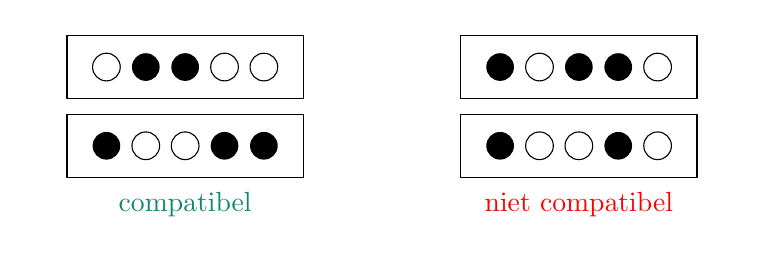
\begin{tikzpicture}[main, line join=bevel]
		\clip (-1,-2) rectangle (8,0.5);
		
		\draw (1,-1.75) node {\color{PineGreen}compatibel};
		\draw (6,-1.75) node {\color{red}niet compatibel};
		
		\draw (-0.5,-0.4) rectangle (2.5,0.4);
		\draw (0,0) circle (5pt);
		\fill (0.5,0) circle (5pt);
		\fill (1,0) circle (5pt);
		\draw (1.5,0) circle (5pt);
		\draw (2,0) circle (5pt);
		
		\begin{scope}[yshift = -1cm]
			\draw (-0.5,-0.4) rectangle (2.5,0.4);
			\fill (0,0) circle (5pt);
			\draw (0.5,0) circle (5pt);
			\draw (1,0) circle (5pt);
			\fill (1.5,0) circle (5pt);
			\fill (2,0) circle (5pt);
		\end{scope}
	
		
	
		\begin{scope}[xshift= 5cm]
			\draw (-0.5,-0.4) rectangle (2.5,0.4);
			\fill (0,0) circle (5pt);
			\draw (0.5,0) circle (5pt);
			\fill (1,0) circle (5pt);
			\fill (1.5,0) circle (5pt);
			\draw (2,0) circle (5pt);
			
			\begin{scope}[yshift = -1cm]
				\draw (-0.5,-0.4) rectangle (2.5,0.4);
				\fill (0,0) circle (5pt);
				\draw (0.5,0) circle (5pt);
				\draw (1,0) circle (5pt);
				\fill (1.5,0) circle (5pt);
				\draw (2,0) circle (5pt);
			\end{scope}
			
		\end{scope}
		
	\end{tikzpicture}
\end{document}
